\documentclass[11pt]{article}

\usepackage[margin=1in]{geometry}
\usepackage{graphicx}
\usepackage{booktabs}
\usepackage{xcolor}
\usepackage{hyperref}
\usepackage{tabularx}
\usepackage{caption}
\usepackage{multirow}

\hypersetup{colorlinks=true, linkcolor=black, urlcolor=blue, citecolor=black}
\setlength{\parskip}{4pt}
\setlength{\parindent}{0pt}

\title{\textbf{Behavioral Error Analysis of LLM-Based Agents:\\
An Agentic Adaptation of \textsc{ErrorMap}}}

\author{Authors withheld}
\date{}

\begin{document}
\maketitle

\begin{abstract}
We adapt \textsc{ErrorMap}~\cite{ashury2026errormap} from
single-shot QA error analysis to long-horizon agent
trajectories, and apply it to 4{,}551 failed sessions produced by
five agent harnesses (\texttt{claude\_code}, \texttt{tool\_calling},
\texttt{tool\_calling\_with\_shortlisting}, \texttt{smolagents\_code},
\texttt{openai\_solo}), five LM backbones (Claude Opus~4.5,
DeepSeek-V3.2, Gemini~3 Pro Preview, GPT-5.2, Kimi-K2.5) and six
benchmarks (\textsc{AppWorld}, \textsc{BrowseCompPlus},
\textsc{SWE-bench}, and three $\tau^2$-bench variants:
airline, retail, telecom). Using GPT-5.5 as judge, we discover a
27-category top-level taxonomy with 2.1\% \emph{Other} coverage and
85\% judge agreement (\textsc{ErrorMap}~paper: 4.8\% / 92\%).
Mapping our categories to the closed taxonomies of
\textsc{ErrorAtlas}-17~\cite{ashury2026errormap} and the
\textsc{AgentErrorTaxonomy}-17~\cite{liu2025agentdebug}, we find
that \textbf{14 categories accounting for 42\% of failures} have no
direct counterpart in either prior taxonomy. The novel categories
are predominantly \emph{control-flow} and \emph{protocol-adherence}
patterns visible only in multi-step trajectories
(e.g.\ \emph{Premature Termination}, \emph{Escalation Handling},
\emph{Diagnostic Protocol Error}, \emph{Looping Behavior},
\emph{Unauthorized Action Execution}). All artifacts---adapted
pipeline, taxonomy, raw trajectories, per-record labels, validation
outputs, and analysis figures---are released publicly.
\end{abstract}

\section{Introduction}

The \textsc{ErrorMap} framework~\cite{ashury2026errormap} extracts
a model-specific failure signature by clustering per-instance error
diagnoses produced by an LLM judge, and aggregates the resulting
labels across 35 datasets and 83 models into the
\textsc{ErrorAtlas}: a hierarchical taxonomy of 17 high-level error
categories. The framework's design assumes the input is a
single-shot prediction (input/output pair plus optional reference);
its prompt is correspondingly QA-flavoured (\emph{``incorrect
response''}, \emph{``model thinking''}, etc.). The
\textsc{AgentErrorTaxonomy}~\cite{liu2025agentdebug} addresses the
agentic setting with a \emph{closed} 17-category schema spanning
five modules (Memory, Reflection, Planning, Action, System) annotated
on 200 trajectories from \textsc{ALFWorld}, \textsc{GAIA}, and
\textsc{WebShop}.

We are interested in the failure modes of \emph{long-horizon
LLM-based agents at scale}---i.e.\ many models and harnesses run on
many benchmarks---and we want a taxonomy that emerges
\emph{bottom-up} from the data rather than being mapped onto a
closed schema. We therefore adapt \textsc{ErrorMap} to ingest
trajectory data, validate it on six benchmarks of practical
interest, and contrast the resulting taxonomy with both prior
schemes.

\section{Methodology}

\subsection{Data}

We collected per-session outputs of the
\href{https://github.com/Exgentic/experiments}{Exgentic} harness:
13{,}652 sessions across the design matrix of five agent
harnesses, five LM backbones, and six benchmarks. We filtered to
sessions marked \texttt{success=False} with at least one executed
step, yielding 4{,}802 candidate failed sessions. After resolving
mirrored \texttt{tool\_calling\_with\_shortlisting} entries (a
post-processing artifact of the harness's CSV pipeline) and
excluding 251 sessions with unresolved CSV/disk session-ID
mismatches, we retained 4{,}551 failures with full trajectory data
(\texttt{trajectory.jsonl}). Of these, 3{,}491 (76.7\%) had at
least one peer-success trajectory available from another agent or
model on the same task, which we use as the \texttt{correct\_outputs}
reference for the judge. The remaining 23\% failed on tasks that no
agent solved (16\% of all tasks were never solved across the
20-attempt design).

For each failed session we assemble a JSONL record containing the
task description, initial environment state (from
\texttt{session.json}), the failed trajectory, the gold trajectory
(if any), and provenance metadata (benchmark, agent, model,
\texttt{run\_id}, \texttt{session\_id}). Trajectories are serialized
as alternating \texttt{[step $n$] ACT}/\texttt{OBS} blocks with
observations truncated to 1{,}500 characters. The full corpus is
142~MB compressed and is released alongside the code.

\subsection{Pipeline adaptation}

We minimally adapt the upstream
\href{https://github.com/IBM/ErrorMap}{\textsc{ErrorMap} repository}:

\begin{enumerate}
\item \textbf{Schema entries.} Add six binary-success entries to
\texttt{dataset2params}, treating any score below~1 as a failure.
\item \textbf{Trajectory adapter.} A 100-line script
(\texttt{scripts/agentic\_csv.py}) converts our JSONL into the per-benchmark
input CSVs \textsc{ErrorMap} expects, with each task contributing
a failure row (\texttt{score}=0) and one peer-success ``gold'' row
(\texttt{score}=1) sharing the same \texttt{example\_id} so that the
\texttt{success\_outputs} lookup in \texttt{single\_error.py} links
them automatically.
\item \textbf{Prompt adaptation.} We rewrite the judge prompt
(\texttt{single\_error\_analysis.j2}) to refer to ``the agent's
trajectory'' rather than ``the model's response'', broaden the
\texttt{error\_summary} guidance to admit reasoning, planning,
tool-use, and control-flow errors as legitimate root causes, swap
the multiple-choice example for an agentic example, and add an
explicit \emph{Label Artifact} branch for cases where the failed
and successful trajectories are behaviorally identical. We also
update the four taxonomy-construction prompts (generation, review,
update, classify) to refer to ``agent failure modes'' and replace
the \emph{Factual Error} example with \emph{Tool Use Error}. No
schema or output-format changes were made.
\end{enumerate}

\subsection{Run configuration}

We use \texttt{azure/gpt-5.5} as the judge with high reasoning
effort, \texttt{max\_workers=100} for concurrent inference, and
\texttt{max\_num\_clusters=25} for the taxonomy construction (the
upstream default; we found that increasing it to~40 \emph{worsened}
coverage by encouraging niche labels rather than broader umbrellas).
The pilot of 100 stratified sessions completed in 6 minutes for
\$5.23 and validated end-to-end behavior. The full run analyzed
4{,}551 sessions in 42 minutes; 35 records (0.8\%) failed due to
proxy rate limiting and were patched with a small targeted re-run.
A second pass over the patched data executed Stage~2 with the
agent-aware taxonomy prompts.

\subsection{Manual cleanup pass}

The first complete run produced 26 top-level categories with
\emph{Other}~$=$~25.8\%, far above the 4.8\% reported by the
\textsc{ErrorMap} paper. Inspection of the records under
\emph{Other} revealed that the recursive clustering had produced
sensible depth-2 sub-categories within \emph{Other}---most of which
were synonyms of existing top-level labels (e.g.\ ``Other/Premature
Termination'' duplicating top-level \emph{Premature Termination}, or
``Other/Information Gathering Error'' being a synonym of top-level
\emph{Evidence Retrieval Omission}). We applied a deterministic
post-processing pass that (a)~promotes depth-2 sub-categories of
\emph{Other} to canonical labels via a hand-curated synonym
mapping, (b)~merges two pairs of overlapping top-level categories
(\emph{Search Recovery Failure}~+ \emph{Search Adaptation Failure};
\emph{Escalation Timing Error}~+ \emph{Escalation Protocol Error}),
and (c)~promotes five distinct depth-2 categories that have no
existing top-level counterpart (\emph{Looping Behavior},
\emph{Planning Error}, \emph{User Communication Error},
\emph{Instruction Following Error},
\emph{State/Goal Tracking Error}). This produced a 27-category
top-level taxonomy with \emph{Other}~$=$~2.1\%, slightly below the
\textsc{ErrorMap} paper's coverage. The mapping is deterministic
and public.

\section{Results}

\subsection{Top-level taxonomy and prevalence}

Table~\ref{tab:prevalence} lists the 22 top-level categories with
$\geq$1\% prevalence (covering 95.7\% of all failures). The
distribution is unusually flat: the largest category
(\emph{Premature Termination}) accounts for only 8.1\% of failures,
and the top~10 categories cumulatively cover 57.5\%. This contrasts
with \textsc{ErrorAtlas}, where the top-five categories
(\emph{Missing Required Element} 15.6\%, \emph{Specification
Misinterpretation} 11.5\%, \emph{Logical Reasoning} 9.1\%,
\emph{Incorrect Identification} 9.0\%, \emph{Computation Error}
8.5\%) cover 53.7\% of failures with a single dominant pattern.
Agent failures, in our corpus, are more diverse.

\begin{table}[h]
\centering
\small
\caption{Top-level failure categories with $\geq$1\% prevalence
(n$=$2{,}868 categorized records). \textbf{Bold} indicates novel
categories not present in either
\textsc{ErrorAtlas}-17~\cite{ashury2026errormap} or
\textsc{AgentErrorTaxonomy}-17~\cite{liu2025agentdebug}.}
\label{tab:prevalence}
\begin{tabular}{rlrr}
\toprule
\# & Category & n & \% \\
\midrule
1 & \textbf{Premature Termination}        & 232 & 8.1 \\
2 & Evidence Retrieval Omission           & 211 & 7.4 \\
3 & \textbf{Search Recovery \& Adaptation}& 183 & 6.4 \\
4 & Unsupported Fabrication               & 167 & 5.8 \\
5 & Tool Invocation Error                 & 167 & 5.8 \\
6 & Constraint Interpretation Error       & 157 & 5.5 \\
7 & \textbf{Escalation Handling}          & 151 & 5.3 \\
8 & Entity Resolution Error               & 143 & 5.0 \\
9 & Evidence Interpretation Error         & 119 & 4.1 \\
10 & \textbf{Diagnostic Protocol Error}    & 118 & 4.1 \\
11 & Action Execution Error                & 118 & 4.1 \\
12 & Candidate Verification Failure        & 115 & 4.0 \\
13 & \textbf{Validation Recovery Failure}  & 104 & 3.6 \\
14 & Quantitative Reasoning Error          & 97  & 3.4 \\
15 & \textbf{Remediation Omission}         & 81  & 2.8 \\
16 & Coverage Enumeration Omission         & 75  & 2.6 \\
17 & \textbf{Finalization Protocol Error}  & 73  & 2.5 \\
18 & \textbf{Unauthorized Action Execution}& 69  & 2.4 \\
19 & Policy Eligibility Error              & 67  & 2.3 \\
20 & \textbf{Query Formulation Error}      & 60  & 2.1 \\
21 & \textbf{Confirmation Handling Error}  & 43  & 1.5 \\
22 & \textbf{Authentication Handling Error}& 36  & 1.3 \\
\midrule
\multicolumn{2}{r}{(Other small categories, n$<$1\%)} & 76 & 2.6 \\
\multicolumn{2}{r}{Other (uncategorized)} & 61 & 2.1 \\
\bottomrule
\end{tabular}
\end{table}

\subsection{Novel categories}

We manually map each of our 27 top-level categories to the closest
fit in \textsc{ErrorAtlas}-17 and \textsc{AgentErrorTaxonomy}-17,
labelling each as ``covered'' (clear synonym in either prior
schema), ``partial overlap'' (loose match), or ``novel'' (no
direct counterpart). Of 27 categories, 6 are covered, 7 partially
overlap, and 14 are novel. The novel categories collectively
account for 1{,}201 records (41.9\% of all categorized failures);
the full mapping is released as
\texttt{taxonomy\_mapping.csv}.

The novel categories cluster into two themes:

\paragraph{Control-flow.} \emph{Premature Termination} (8.1\%)
captures volitional early stops---agents that call \texttt{finish()}
or send a closing message before completing required work. Its
nineteen depth-2 sub-categories distinguish, e.g.\ stopping during
diagnosis (\emph{Diagnostic Follow-through}, 18 records), stopping
before applying a fix (\emph{Code Implementation}, 14), abandoning
search prematurely (\emph{Search Persistence}, 22), and stopping
mid-batch (\emph{Batch Iteration}, 3). Volitional early stops are
distinct from \textsc{AgentErrorTaxonomy}'s \emph{Step Limit
Exhaustion} (a System category for budget-driven failures) and from
\textsc{ErrorAtlas}'s \emph{Missing Required Element} (which
describes output omissions).
\emph{Looping Behavior} (0.4\%) captures action repetition without
progress---a multi-step pattern with no QA analogue.
\emph{Validation Recovery Failure} (3.6\%) and \emph{Search Recovery
\& Adaptation} (6.4\%) capture failure of post-error adaptation,
which the prior schemas group under broader Reflection or Planning
modules.

\paragraph{Protocol adherence.} Several novel categories describe
violations of explicit task or domain protocols:
\emph{Escalation Handling} (5.3\%) for escalating too early or too
late, \emph{Diagnostic Protocol Error} (4.1\%) for skipping the
required user-side diagnostic dialogue, \emph{Confirmation
Handling Error} (1.5\%) for bypassing required user confirmations,
\emph{Authentication Handling Error} (1.3\%) for credential
misuse, and \emph{Unauthorized Action Execution} (2.4\%) for
performing actions the user did not approve. These categories are
heavily represented in $\tau^2$-bench (which has explicit policy
documents) but the same patterns appear in domain-policy-laden
trajectories elsewhere.

\subsection{Per-model failure signatures}

The same five LM backbones produce visibly different failure
mixes despite comparable end-task accuracy
(Figure~\ref{fig:per-model}). Selected distinctive top-3 patterns:

\begin{itemize}
\item \textbf{DeepSeek-V3.2:} \emph{Premature Termination} (7.9\%)
and \emph{Search Recovery \& Adaptation} (\textit{combined patterns}); gives up
relatively easily.
\item \textbf{Kimi-K2.5:} \emph{Unsupported Fabrication} (7.2\%),
\emph{Tool Invocation Error} (6.4\%), \emph{Action Execution
Error} (6.4\%); sloppy execution and confabulation.
\item \textbf{GPT-5.2:} \emph{Escalation Timing Error} (8.4\%
pre-merge), \emph{Premature Termination} (7.8\%); escalates too
soon.
\item \textbf{Claude Opus~4.5:} \emph{Candidate Verification
Failure} (7.3\%), \emph{Diagnostic Protocol Error} (6.3\%); methodical
investigation but stops short of the fix.
\item \textbf{Gemini~3 Pro Preview:} \emph{Unsupported Fabrication}
(5.7\%), \emph{Search Adaptation Failure} (5.2\%); confabulates
when search underperforms.
\end{itemize}

These distinctive signatures echo the central
\textsc{ErrorMap}~\cite{ashury2026errormap} thesis: aggregate
accuracy hides systematic differences in \emph{how} models fail.

\begin{figure}[h]
\centering
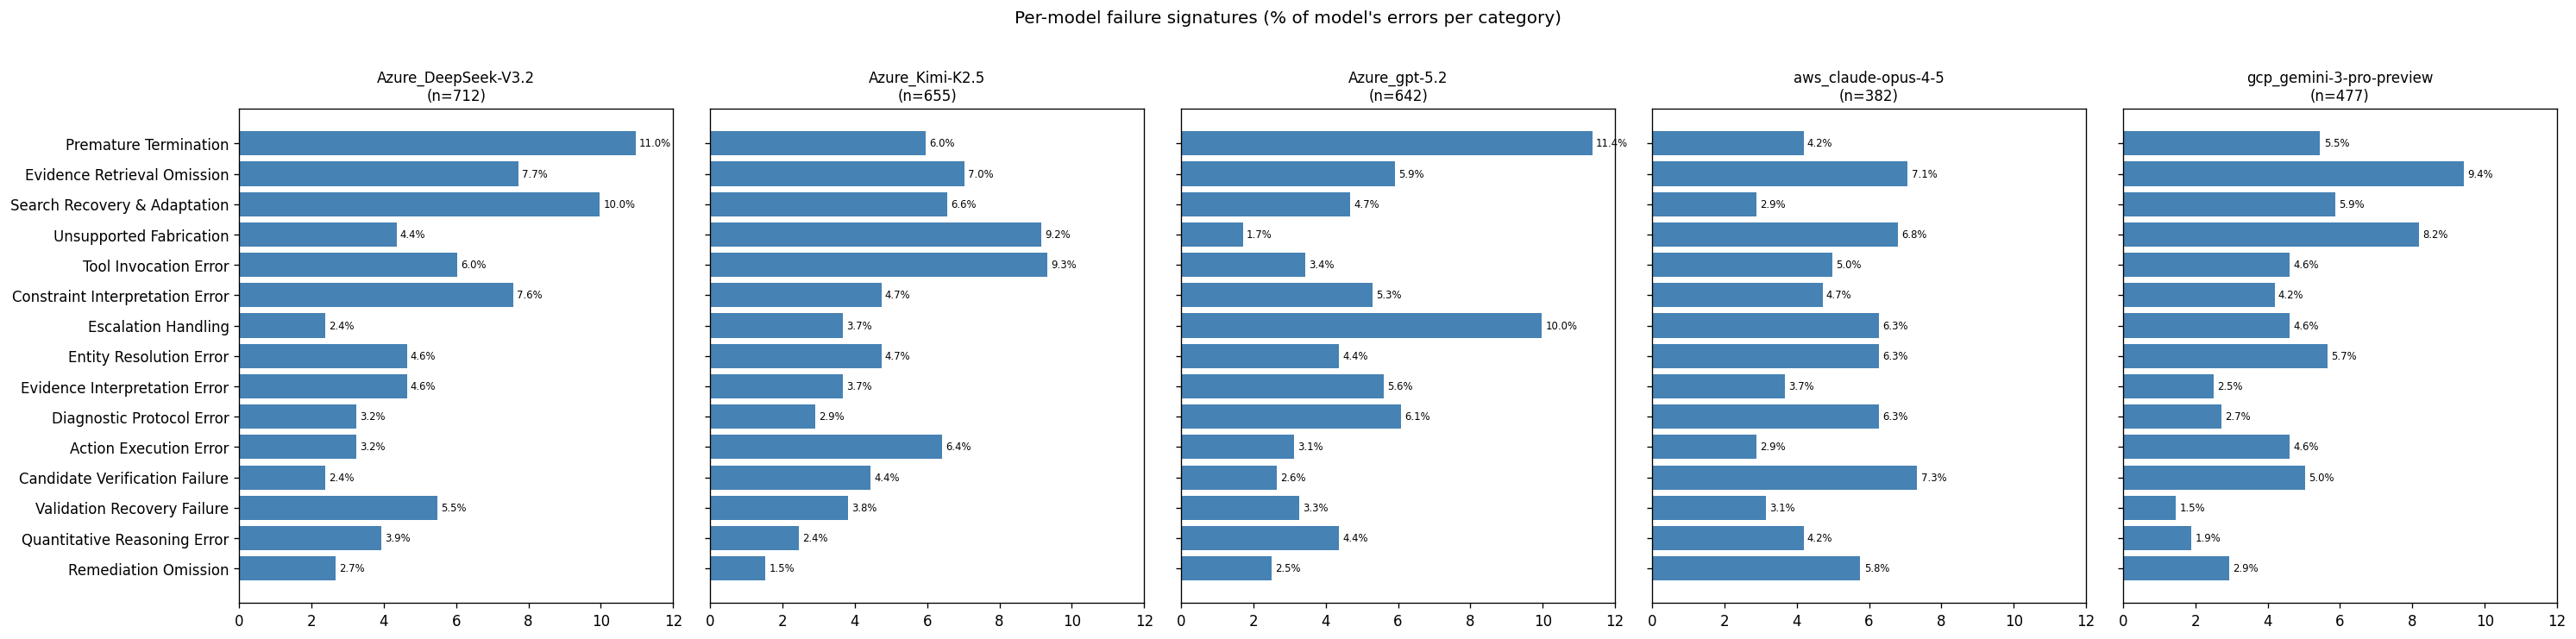
\includegraphics[width=\textwidth]{per_model_signatures.png}
\caption{Per-model failure signatures (top-15 categories,
column-normalized).}
\label{fig:per-model}
\end{figure}

\subsection{Per-agent and per-benchmark variation}

Per-agent (harness) breakdowns show smaller spread than per-model
breakdowns, with \texttt{tool\_calling} and
\texttt{tool\_calling\_with\_shortlisting} producing nearly
identical signatures---consistent with their shared
post-processing CSV in the upstream Exgentic harness, which
mirrors one to the other for non-AppWorld benchmarks.
\texttt{smolagents\_code} differs in placing \emph{Search
Adaptation Failure} highest, consistent with code-execution-style
agents that retry rather than redirect. Per-benchmark variation
is large: \textsc{SWE-bench} dominates \emph{Premature Termination}
(agents stop before applying a patch) while
$\tau^2$-airline/retail/telecom dominate \emph{Escalation Handling}
and \emph{Confirmation Handling Error}. See
\texttt{breakdown\_\{model,agent,benchmark\}.csv} and the
\texttt{crosstab\_\{...\}.png} heatmaps for the full picture.

\subsection{Judge accuracy validation}

Following \textsc{ErrorMap}'s validation protocol, we sample 100
labelled records and ask the judge to discriminate the assigned
category (with description) from a randomly-drawn alternative
category, in a forced-choice setting with order randomized. The
judge prefers the assigned label \textbf{85 of 100 times} (vs.\
92\% in the \textsc{ErrorMap}~paper). The lower agreement is
plausibly attributable to (a)~our larger 27-category vocabulary vs.\
the paper's 17~categories, increasing the likelihood that
randomly-drawn negatives are semantically close, and (b)~the longer
input contexts inherent to trajectories. Agreement of 85\% is
nonetheless substantial and exceeds chance by an order of magnitude.

\section{Discussion}

\subsection{What's contributed}

We make three contributions. First, a minimal, defensible
adaptation of the \textsc{ErrorMap} pipeline to long-horizon
agent trajectories, which we release on a public fork. Second,
the assembled corpus of 4{,}551 failed trajectories paired with
peer-success trajectories from the Exgentic harness, the largest
such collection we are aware of, also released. Third, a 27-category
top-level taxonomy of agent failures with detailed sub-categories,
mapped against \textsc{ErrorAtlas}-17 and
\textsc{AgentErrorTaxonomy}-17, with 14 novel categories that
collectively explain 42\% of failures. The novel categories are
predominantly control-flow and protocol-adherence patterns
visible only in multi-step trajectories.

\subsection{Limitations}

(i)~Our taxonomy is judge-LLM-derived; the validation accuracy
is below the \textsc{ErrorMap} paper's 92\%. Tighter validation
(human spot-check, dual-judge agreement) would strengthen claims.
(ii)~Manual post-processing was applied to merge synonyms and
promote unrecognized novel patterns; while the mapping is
deterministic and public, an algorithmic version would be
preferable. (iii)~Increased \texttt{max\_num\_clusters} from 25 to
40 worsened coverage rather than improved it---we do not have a
principled explanation for this and treat the original setting as
canonical. (iv)~$\tau^2$-bench is over-represented relative to the
other benchmarks because it contributes the most failures with
gold peers; this skews the prevalence of policy-related categories.

\subsection{Reproducibility}

All artifacts are released:
\begin{itemize}
\item Adapted pipeline code:
\href{https://github.com/elronbandel/ErrorMap/tree/agentic-trajectories}{elronbandel/ErrorMap @ agentic-trajectories}
\item Trajectory dataset (676~MB JSONL, 142~MB compressed):
release \texttt{agentic-data-v1} on the same fork.
\item Final analysis CSVs and figures: \texttt{analysis/} on the
same branch (this document is \texttt{analysis/paper.tex}).
\end{itemize}

\section{Conclusion}

Adapting an off-the-shelf failure-analysis pipeline to a new domain
required modest engineering---updates to thresholds, a trajectory
adapter, and a vocabulary swap in five Jinja2 templates---and
produced agent-specific findings that materially extend prior
taxonomies. The dominant failure patterns of long-horizon agents are
not the dominant failure patterns of single-shot QA: they are
instead about \emph{when to stop}, \emph{how to recover}, and
\emph{whether to follow a protocol}. We release everything required
to reproduce this analysis or extend it to new agent harnesses,
benchmarks, or judges.

\bibliographystyle{plain}
\begin{thebibliography}{9}

\bibitem{ashury2026errormap}
Shir Ashury-Tahan, Yifan Mai, Elron Bandel, Michal Shmueli-Scheuer,
Leshem Choshen.
\emph{ErrorMap and ErrorAtlas: Charting the Failure Landscape of
Large Language Models.}
arXiv:2601.15812, 2026.

\bibitem{liu2025agentdebug}
Anonymous (ICLR 2026 submission).
\emph{Where LLM Agents Fail and How They Can Learn from Failures.}
arXiv:2509.25370, 2025.

\bibitem{cemri2025mast}
Mert Cemri, Melissa Z. Pan, Shuyi Yang, et al.
\emph{Why Do Multi-Agent LLM Systems Fail?}
arXiv:2503.13657, 2025.

\bibitem{aiweb2025hal}
Boyi Wei, et al.
\emph{HAL: Holistic Agent Leaderboard.}
arXiv:2510.11977, 2025.

\end{thebibliography}

\end{document}
